\documentclass{amsart}

%%%%%%%%%%%%%%%

\usepackage[utf8]{inputenc}
% \usepackage[spanish]{babel}
% \usepackage[top=1in, bottom=1in, left=1.2in, right=1.2in]{geometry}
\usepackage{amssymb}
\usepackage{amsmath}
\usepackage{amsfonts}
\usepackage{amsthm}
\usepackage{wasysym}
\usepackage{enumitem}
\usepackage{listings}
\usepackage{xcolor}
\usepackage{tikz}

% sets
\newcommand{\NN}{\mathbf{N}}
\newcommand{\ZZ}{\mathbf{Z}}
\newcommand{\QQ}{\mathbf{Q}}
\newcommand{\RR}{\mathbf{R}}
\newcommand{\Zpos}{\ZZ^{+}}
\newcommand{\Rpos}{\RR^{+}}

% brackets
\newcommand{\la}{\langle}
\newcommand{\ra}{\rangle}

% formal statements
\newtheorem{prop}{Proposition}

\theoremstyle{plain}
\newtheorem{clm}{Claim}

\theoremstyle{definition}
\newtheorem{defn}{Definition}

\newtheorem{exl}{Example}

\theoremstyle{remark}
\newtheorem{rmk}{Remark}

% display of code
\definecolor{oliveGreen}{rgb}{0.13,0.55,0.13}
\lstset{%
    language = Java,
    basicstyle = \normalsize\ttfamily,
    keywordstyle = \bf,
    commentstyle = \color{oliveGreen}\it,
    stringstyle = \color{blue},
    showstringspaces = false,
    columns = fullflexible%
}


\title{isis1105 \\ definiciones tarea 4}
\author{sección 3}
% \date{\today}

\begin{document}

\maketitle

\section{Basics} 

\begin{defn}
    A \emph{graph} is a pair $\la N, A \ra$ such that $A$ consists of subsets of $N$ of size 2. We call $N$ the set of \emph{nodes} and $A$ the set of \emph{edges}.
\end{defn}

\begin{defn}
    Let $G = \la N,A \ra$ be a graph.
    \begin{enumerate}
        \item The \emph{order} of $G$ is $\#N$.
        \item The \emph{degree} of $v \in N$ is $\# \{e \in A \ | \ v  \in e\}$.
    \end{enumerate}
\end{defn}

\begin{exl}
    Let $N = \{ 1, 2, 3 \}$ and let $A = \{ \{ 1, 2 \}, \{ 1, 3 \} \}$. Then $\la N, A \ra$ can be dawn as

    \begin{center}
        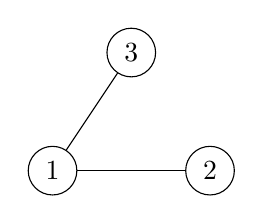
\begin{tikzpicture}
            % Nodes
            \node[circle,draw] (1) at (0,0) {1};
            \node[circle,draw] (2) at (2,0) {2};
            \node[circle,draw] (3) at (1,1.5) {3};

            % Edges
            \draw (1) -- (2);
            \draw (1) -- (3);
        \end{tikzpicture}
    \end{center}

    Node 1 has degree 2, and the other nodes have degree 1.

    If now $A' =\{ \{ 1, 2 \}, \{ 1, 3 \}, \{ 2, 3 \} \}$, then $\la N, A' \ra$ can be drawn as

    \begin{center}
        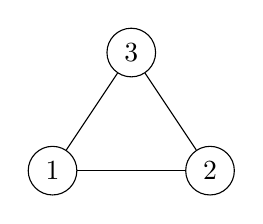
\begin{tikzpicture}
            % Nodes
            \node[circle,draw] (1) at (0,0) {1};
            \node[circle,draw] (2) at (2,0) {2};
            \node[circle,draw] (3) at (1,1.5) {3};

            % Edges
            \draw (1) -- (2);
            \draw (1) -- (3);
            \draw (2) -- (3);
        \end{tikzpicture}
    \end{center}

    Now all three nodes have degree 2.

\end{exl}

\begin{defn}
    \begin{enumerate}
        \item[]
        \item A $k-$\emph{path} is a sequence of nodes $\mathbf{p} = v_0,...,v_{k-1},v_{k}$ Such that $v_i \neq v_j$  and $\{v_i, v_{i+1}\} \in A$ for all $i = 0,...,k-1$. We also say that $\mathbf{p}$ is a $v_0v_k-$path of length $k$, since it involves that many edges. % k is the nr. of nodes in the path.
        \item A $k-$\emph{cycle} is a sequence of nodes $\mathbf{c} = v_0,...,v_{k-2},v_{k-1}$ Such that $v_i \neq v_j$ except for $v_0 = v_{k-1}$, and $\{v_i, v_{(i+1) \, \mathbf{mod} \, k}\} \in A$ for all $i = 0,...,k-1$.
    \end{enumerate}
    
\end{defn}

\begin{defn}
    \begin{enumerate}
        \item[] 
        \item The nodes $u,v$ are said to be \emph{connected} if they are equal or there exists a $uv-$path, and we denote this by $u \sim v$. Notice that the resulting relation $\sim$ is an equivalence relation. Given the node $u$, its \emph{connected component} is the subgraph induced by the edges connected to it. We use the notation $C_u$ for the connected component of the node $u$.
        \item[] 
        \item In general $G = C_{u_1} \sqcup C_{u_2} \sqcup ... \sqcup C_{u_t}$ with $1 \leq t \leq n$, where $n$ is the order of $G$. Namely, a graph is the disjoint union of the connected components of its nodes. We also say that ``$C_v$ is a connected component of $G$".
        \item[] 
        \item The graph $G$ is said to be \emph{connected} if there exists a path between any two different nodes. Equivalently, $G$ has a single connected component. If $G$ has $n$ nodes called $0,1,\dots,n-1$ and is connected, then $G = C_0 = C_1 = \dots = C_{n-1}$.
    \end{enumerate}
\end{defn}

\begin{exl}
    Let $G = \la N, A \ra$ with
    $$
    \begin{cases}
        N = \{0, 1, \dots, 8\}. \\
        A = \{ \{0,1\}, \, \{2,3\}, \, \{2,4\}, \, \{3,4\}, \, \{5,6\}, \\
            \ \ \ \ \ \ \ \ \{5,7\}, \, \{6,7\}, \, \{6,8\}, \, \{7,8\}, \}.
    \end{cases}
    $$
    Then $G$ has three connected components: 
    \begin{eqnarray*}
        C_0 = C_1 \\
        C_2 = C_3 = C_4 \\
        C_5 = C_6 = C_7 = C_8
    \end{eqnarray*}
    This can be visualized in the following picture of $G$:

    \bigskip
    
    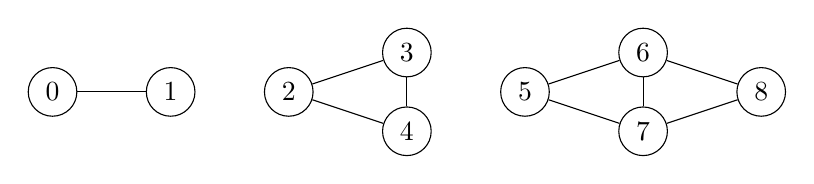
\begin{tikzpicture}[node distance=1.5cm]
        % First component with 2 nodes
        \node[circle, draw] (0) at (0,0) {0};
        \node[circle, draw] (1) at (1.5,0) {1};
        \draw (0) -- (1);
        
        % Second component with 3 nodes
        \node[circle, draw] (2) at (3,0) {2};
        \node[circle, draw] (3) at (4.5,0.5) {3};
        \node[circle, draw] (4) at (4.5,-0.5) {4};
        \draw (2) -- (3);
        \draw (2) -- (4);
        \draw (3) -- (4);
        
        % Third component with 4 nodes
        \node[circle, draw] (5) at (6,0) {5};
        \node[circle, draw] (6) at (7.5,0.5) {6};
        \node[circle, draw] (7) at (7.5,-0.5) {7};
        \node[circle, draw] (8) at (9,0) {8};
        \draw (5) -- (6);
        \draw (5) -- (7);
        \draw (6) -- (7);
        \draw (6) -- (8);
        \draw (7) -- (8);
    \end{tikzpicture}
    
    \bigskip
    \bigskip
    
    The degrees of the nodes are 
    \begin{eqnarray*}
        \deg(0) = \deg(1) = 1 \\
        \deg(2) = \deg(3) = \deg(4) = \deg(5) = \deg(8) = 2 \\
        \deg(6) = \deg(7) = 3.
    \end{eqnarray*}
    
\end{exl}


\begin{defn}
    A graph is \emph{acyclic} if there is at most one path joining any two different nodes.
\end{defn}

\end{document}